% Options for packages loaded elsewhere
\PassOptionsToPackage{unicode}{hyperref}
\PassOptionsToPackage{hyphens}{url}
%
\documentclass[
]{article}
\usepackage{amsmath,amssymb}
\usepackage{lmodern}
\usepackage{iftex}
\ifPDFTeX
  \usepackage[T1]{fontenc}
  \usepackage[utf8]{inputenc}
  \usepackage{textcomp} % provide euro and other symbols
\else % if luatex or xetex
  \usepackage{unicode-math}
  \defaultfontfeatures{Scale=MatchLowercase}
  \defaultfontfeatures[\rmfamily]{Ligatures=TeX,Scale=1}
\fi
% Use upquote if available, for straight quotes in verbatim environments
\IfFileExists{upquote.sty}{\usepackage{upquote}}{}
\IfFileExists{microtype.sty}{% use microtype if available
  \usepackage[]{microtype}
  \UseMicrotypeSet[protrusion]{basicmath} % disable protrusion for tt fonts
}{}
\makeatletter
\@ifundefined{KOMAClassName}{% if non-KOMA class
  \IfFileExists{parskip.sty}{%
    \usepackage{parskip}
  }{% else
    \setlength{\parindent}{0pt}
    \setlength{\parskip}{6pt plus 2pt minus 1pt}}
}{% if KOMA class
  \KOMAoptions{parskip=half}}
\makeatother
\usepackage{xcolor}
\IfFileExists{xurl.sty}{\usepackage{xurl}}{} % add URL line breaks if available
\IfFileExists{bookmark.sty}{\usepackage{bookmark}}{\usepackage{hyperref}}
\hypersetup{
  pdftitle={Methods},
  hidelinks,
  pdfcreator={LaTeX via pandoc}}
\urlstyle{same} % disable monospaced font for URLs
\usepackage[margin=1in]{geometry}
\usepackage{longtable,booktabs,array}
\usepackage{calc} % for calculating minipage widths
% Correct order of tables after \paragraph or \subparagraph
\usepackage{etoolbox}
\makeatletter
\patchcmd\longtable{\par}{\if@noskipsec\mbox{}\fi\par}{}{}
\makeatother
% Allow footnotes in longtable head/foot
\IfFileExists{footnotehyper.sty}{\usepackage{footnotehyper}}{\usepackage{footnote}}
\makesavenoteenv{longtable}
\usepackage{graphicx}
\makeatletter
\def\maxwidth{\ifdim\Gin@nat@width>\linewidth\linewidth\else\Gin@nat@width\fi}
\def\maxheight{\ifdim\Gin@nat@height>\textheight\textheight\else\Gin@nat@height\fi}
\makeatother
% Scale images if necessary, so that they will not overflow the page
% margins by default, and it is still possible to overwrite the defaults
% using explicit options in \includegraphics[width, height, ...]{}
\setkeys{Gin}{width=\maxwidth,height=\maxheight,keepaspectratio}
% Set default figure placement to htbp
\makeatletter
\def\fps@figure{htbp}
\makeatother
\setlength{\emergencystretch}{3em} % prevent overfull lines
\providecommand{\tightlist}{%
  \setlength{\itemsep}{0pt}\setlength{\parskip}{0pt}}
\setcounter{secnumdepth}{5}
\newlength{\cslhangindent}
\setlength{\cslhangindent}{1.5em}
\newlength{\csllabelwidth}
\setlength{\csllabelwidth}{3em}
\newlength{\cslentryspacingunit} % times entry-spacing
\setlength{\cslentryspacingunit}{\parskip}
\newenvironment{CSLReferences}[2] % #1 hanging-ident, #2 entry spacing
 {% don't indent paragraphs
  \setlength{\parindent}{0pt}
  % turn on hanging indent if param 1 is 1
  \ifodd #1
  \let\oldpar\par
  \def\par{\hangindent=\cslhangindent\oldpar}
  \fi
  % set entry spacing
  \setlength{\parskip}{#2\cslentryspacingunit}
 }%
 {}
\usepackage{calc}
\newcommand{\CSLBlock}[1]{#1\hfill\break}
\newcommand{\CSLLeftMargin}[1]{\parbox[t]{\csllabelwidth}{#1}}
\newcommand{\CSLRightInline}[1]{\parbox[t]{\linewidth - \csllabelwidth}{#1}\break}
\newcommand{\CSLIndent}[1]{\hspace{\cslhangindent}#1}
\usepackage{booktabs}
\usepackage{longtable}
\usepackage{array}
\usepackage{multirow}
\usepackage{wrapfig}
\usepackage{float}
\usepackage{colortbl}
\usepackage{pdflscape}
\usepackage{tabu}
\usepackage{threeparttable}
\usepackage{threeparttablex}
\usepackage[normalem]{ulem}
\usepackage{makecell}
\usepackage{xcolor}
\ifLuaTeX
  \usepackage{selnolig}  % disable illegal ligatures
\fi

\title{Methods}
\author{}
\date{\vspace{-2.5em}}

\begin{document}
\maketitle

\hypertarget{site}{%
\subsection{Site}\label{site}}

The study site was located at the Michigan State University (MSU) - Detroit Partnership for Food, Learning, and Innovation (DPFLI) (42.4, -83.3), a 1.6-ha (4 acres) extension facility dedicated to urban agriculture and engaging with local small-scale growers in Detroit, MI, USA.
The climate is temperate with four seasons, with mean annual temperature of \textasciitilde9.5 C (49.1 F) and precipitation at \textasciitilde787 mm (31 in) (\url{ncdc.noaa.gov}).
The site was formerly a school building and associated playground until 2016 when it was demolished after closing due to low funding and the land became vacant.
The habitat is \textasciitilde1.2 km (\textasciitilde0.8 mi) away from a small river, conferring some wetland ecosystem properties like denser soils.
It is also surrounded by sealed sidewalk and small roads on all four sides, which likely affects runoff and drainage patterns (Fig \ref{fig:plots}a).

\begin{verbatim}
## $`1`
\end{verbatim}

\begin{figure}
\centering
\includegraphics{meth_files/figure-latex/plots-1.pdf}
\caption{\label{fig:plots-1}Field site images (a) map data © 2022 USDA-NRCS SSURGO web soil survey showing likely soil class division given field and lab data, (b) soil profile from North-East site area near current education center, (c) plot layout design, and (d) aerial drone view of treated study area plots. Photo credits: (b) Naim Edwards, (d) Edgar Cardenas.}
\end{figure}

\begin{verbatim}
## 
## $`2`
\end{verbatim}

\begin{figure}
\centering
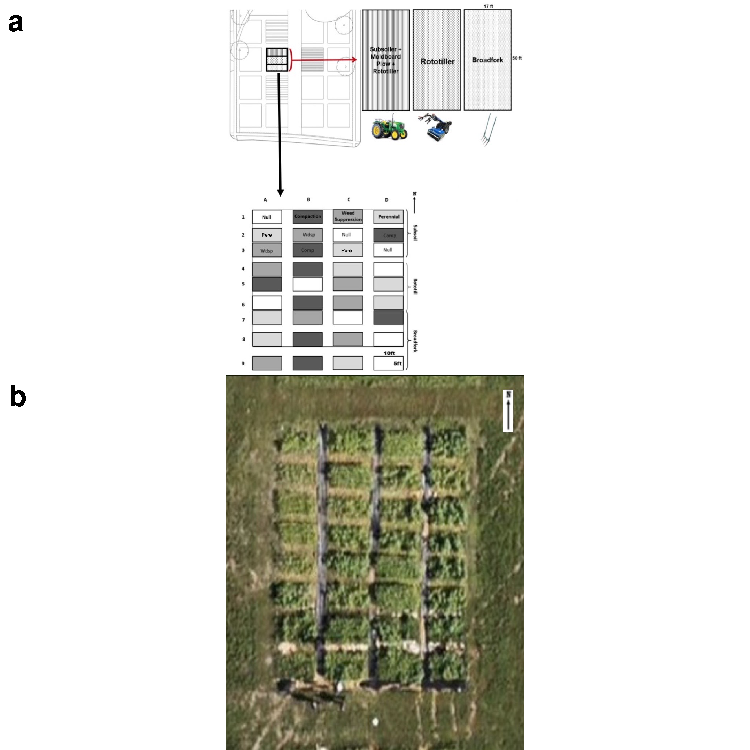
\includegraphics{meth_files/figure-latex/plots-2.pdf}
\caption{\label{fig:plots-2}Field site images (a) map data © 2022 USDA-NRCS SSURGO web soil survey showing likely soil class division given field and lab data, (b) soil profile from North-East site area near current education center, (c) plot layout design, and (d) aerial drone view of treated study area plots. Photo credits: (b) Naim Edwards, (d) Edgar Cardenas.}
\end{figure}

\begin{verbatim}
## 
## attr(,"class")
## [1] "list"      "ggarrange"
\end{verbatim}

Site soils can be classified as Technosols (Fig \ref{fig:plots}b), given that large metal artifacts can be found throughout various profiles \emph{(\protect\hyperlink{ref-fao14}{FAO 2014})}, from when the area was filled in with nearby soils during highway road construction, as was common in mid-western USA industrial manufacturing cities many decades ago in the \emph{1960s} \emph{(\protect\hyperlink{ref-beniston16}{Beniston, Lal, and Mercer 2016})}.
Accordingly, the growing area has both a finer- and coarser-textured side (Fig \ref{fig:plots}a),
and this study was done on the side with consistent clay of \textasciitilde37\%.
Topsoil A horizons are 1-2'' (\textless5 cm) deep, and subsoil B horizons can be \textgreater30.5 cm (1 ft) deep, with a muted yellow color 10YR 8/4 (Fig \ref{fig:plots}b).
A baseline site-level soil lab assessment determined that the top \emph{4 in (10 cm)} of soils around the site together have relatively good organic matter at
\textasciitilde2.5 ±
0.3\%
and nutrient levels, including concentrations of heavy metals like lead and arsenic which were present below harmful government human-contact standards (\url{cfpub.epa.gov/ecotox}).
Site soils were also assesed to have decent but sub-optimal \emph{CO\textsubscript{2}} respiration rates of
0.2 ±
0.04 mg per day
(Table \ref{tab:chemKbl}).
Initial main concerns limiting productivity include high alkaline pH of
8.1 ±
0.1,
lowering availability of existing nutrients, as well as weak aggregate stability of
19 ±
4.4,
leading to concerns with aeration, infiltration, rooting, crusting when dry, erosion, and runoff (Table \ref{tab:chemKbl}).

\begin{longtable}[]{@{}ccccc@{}}
\caption{\label{tab:chemKbl}Baseline Soil Health Assessment (Cornell, Ithaca, NY, USA)}\tabularnewline
\toprule
Kind & Variable & Median (n=10) & Deviation & Descriptor \\
\midrule
\endfirsthead
\toprule
Kind & Variable & Median (n=10) & Deviation & Descriptor \\
\midrule
\endhead
Biological & Organic Matter (\%) & 2.5 & 0.3 & Very Low \\
& Respiration (mg per day) & 0.2 & 0.0 & Medium \\
Physical & Aggregate Stability (\%) & 19.0 & 4.4 & Very Low \\
Chemical & pH & 8.1 & 0.1 & Poor \\
& Phosphorus (ppm) & 2.2 & 1.0 & Medium \\
& Potassium (ppm) & 103.8 & 36.3 & Optimal \\
& Iron (ppm) & 6.0 & 4.4 & Optimal \\
& Magnesium (ppm) & 463.6 & 24.9 & Optimal \\
& Manganese (ppm) & 42.1 & 4.9 & Optimal \\
& Zinc (ppm) & 3.8 & 2.9 & Optimal \\
& Heavy metals (Pb, Al, As, Cu) & - & - & Safe \\
\bottomrule
\end{longtable}

\hypertarget{design}{%
\subsection{Design}\label{design}}

The study area was a 278 \emph{m\textsuperscript{2}} (2992.4 \emph{ft\textsuperscript{2}}) section on the East side of the site under the former school building that was divided into 36 separate 4.6 \emph{m\textsuperscript{2}} (49.5 \emph{ft\textsuperscript{2}}) plots in nine rows and four columns (Fig \ref{fig:plots}c).
Tillage groups spanned the nine columns in adjacent groups of three, while cover crop mix treatments spanned the rows with one row per cover crop mix, totaling 36 plots, or 12 plots per tillage group and nine plots per cover crop mix.
Before applying treatments, approximately 0.2 \emph{m\textsuperscript{3}} (8.5 \emph{ft\textsuperscript{3}}) of compost was incorporated into each plot.

Tillage treatments represented methods of increasing intensity available for small scale agriculture, also varying in cost, machinery needed, and sometimes grower preferences \emph{(\protect\hyperlink{ref-drugova22}{Drugova, Curtis, and Ward 2022})}.
Specifially, treatments included no-till with a broadfork \emph{(NT)}, roto-tiller \emph{(RT)}, and tractor-till \emph{(TT)} with implements.
Tractor-till plots were worked with a subsoiler, moldboard plow, and roto-tiller attached to a tractor up to 30.5 cm (1 ft) deep.
Roto-till plots were treated with a rototiller implement up to 20 cm (7.9 in) deep.
Lastly, no-till plots were worked with only a broadfork up to 10 cm (3.9 in) deep.
All tilling was done once early in the season after one typical compost application and before planting cover crops.

Cover crop mixes were designed primarily based on plants associated with targeted benefits, and as possible, relative simplicity of re-seeding and winter-kill (e.g.~more heat tolerant) \emph{(\protect\hyperlink{ref-clark07}{Clark 2007})}.
Three mixes were designed to target three functions, with each mix containing three different plant species (Table \ref{tab:crops}).
The mix specifically designed to alleviate compaction generally focused on plants with roots that tend to penetrate and loosen soil well, and ultimately included
crimson clover (\emph{Trifolium incarnatum}),
forage radish (\emph{Raphanus sativus var. longipinnatus}), and
cereal ryegrass (\emph{Secale cereale})
.
The mix targeting weed suppression included heat- and drought-tolerant crops that tend to grow rapidly, allowing them to outcompete other plants--the taxa chosed were
sorghum-sudangrass (\emph{Sorghum bicolor x Sorghum bicolor var. sudanese}),
cowpea/black-eyed pea (\emph{Vigna unguiculata subsp. unguiculata}), and
buckwheat (\emph{Fagopyrum esculentum}).
Lastly, a mix was dedicated to perennial cover crops, which in contrast to annuals can survive the winter and thus tend to accumulate biomass and establish before spring weeds--this mix included
hairy vetch (\emph{Vicia villosa}),
red clover (\emph{Trifolium pratense}), and
wheat (\emph{Triticum aestivum}).
We also had a null control group consisting of established vegetation within the plot, where no additional seeds were sown.

\begin{longtable}[]{@{}ccc@{}}
\caption{\label{tab:crops}Cover crop mixes}\tabularnewline
\toprule
Function & Plants & Binomial \\
\midrule
\endfirsthead
\toprule
Function & Plants & Binomial \\
\midrule
\endhead
Weed Suppression & Sorghum-Sudangrass & Sorghum bicolor x S. bicolor var. sudanese \\
& Cowpea/Black-Eyed Pea & Vigna unguiculata subsp. unguiculata \\
& Buckwheat & Fagopyrum esculentum \\
Perennial & Hairy Vetch & Vicia villosa \\
& Red Clover & Trifolium pratense \\
& Wheat & Triticum aestivum \\
Compaction & Forage Radish & Raphanus sativus var. longipinnatus \\
& Crimson Clover & Trifolium incarnatum \\
& Cereal Ryegrass & Secale cereale \\
Null & Existing vegetation (no manipulation) & - \\
\bottomrule
\end{longtable}

\hypertarget{sampling}{%
\subsection{Sampling}\label{sampling}}

Soil compaction was measured with a penetrometer \emph{(AgraTronix \#08180)} in four randomly selected spots within each quarter of every plot, as the depth where resistance was 2 MPa (290.1 psi, \emph{lbs in\textsuperscript{-2}}), which is considered hardpan that roots typically cannot penetrate \emph{(\protect\hyperlink{ref-correa19}{Correa et al. 2019})}.
Measurements were recorded to the nearest \emph{2.5 cm (1 inch)} on dry days.

Soil water infiltration down to \emph{10}
cm \emph{(8.75 in)} depth was measured using a 16.5 \emph{(9.5 in)} wide aluminum cylinder, set away from dense vegetation and any impeding large roots, and recording the time up to 160 sec for \emph{1 L (32 fl oz)} to pass through, representing a typical local rainfall onto \textasciitilde0.10 \emph{m\textsuperscript{2}} (\textasciitilde1 \emph{ft\textsuperscript{2}}) of soil area (\url{waterdata.usgs.gov}).

Weed pressure was measured using percent cover, richness, and density, following similar studies \emph{(\protect\hyperlink{ref-storkey18}{Storkey and Neve 2018})}.
Weed cover was estimated as the total proportion of plot area covered by any weed biomass, descretized into intervals of ten.
Weed richness, a measure of diversity, was recorded by counting the number of unique morphospecies observed in each plot.
Finally, weed density was measured as the number of stems of either of the two most abundant weed taxa, pigweed (\emph{Amaranthus viridis}) and velvetleaf (\emph{Abutilon theophrasti}), also descretized into intervals of ten up to 50 stems per plot.

Five forage radish (Brassica \emph{Raphanus sativus var. longipinnatus}) roots were randomly selected from each plot in the compaction treatment and measured for length, individually, and wet weight, as a cluster.
The length of a radish root was measured from the hypocotyl, or root cap, to where the root became \textasciitilde6.3 mm (\textasciitilde1⁄4 in) wide.

Sampling was done in July and October 2019 and the following Spring.

\hypertarget{statistics}{%
\subsection{Statistics}\label{statistics}}

Field space limited strict plot replication for treatment combinations (\emph{n}=3), and thus inference from advanced nested mixed models \emph{(\protect\hyperlink{ref-silk20}{Silk, Harrison, and Hodgson 2020})}, so analysis focused on specific hypotheses tested using simpler, more conservative non-parametric tests that make few underlying assumptions about data and thus appropriate for data with lower replication.
Kruskal-Wallis tests were run for tillage and cover crop treatments separately, with alpha corrections from 0.05 to 0.01 under multiple comparisons to descriptively parse any treatment interactions, and overall significant treatment effects were followed up by post-hoc Wilcoxon pairwise tests with Holm-corrected p-value adjustments.
All data were centered at plot-level medians, often more robust than means, and where applicable pooled across sampling times given no preliminary significant variation along this axis, together with minimal relevance to focal hypotheses in field studies \emph{(\protect\hyperlink{ref-davies15b}{Davies and Gray 2015})}, and was a general solution to uneven sampling across response variables, minimally increasing statistical power (\emph{n}\textgreater3-6).
For clarity, results figures were designed to reflect statistical models and grouping transparently.
Significant treatment effect sizes were estimated with \emph{eta\textsuperscript{2}} \emph{(\protect\hyperlink{ref-tomczak14}{Tomczak and Tomczak 2014})} and raw median differences at finer pairwise levels.
All calculations and analyzes were done in R version 4.2.0 (2022-04-22) \emph{(\protect\hyperlink{ref-base}{R Core Team 2022})} with useful functions from the packages \emph{tidyverse} 1.3.1 \emph{(\protect\hyperlink{ref-tidyverse}{Wickham et al. 2019})}, \emph{rstatix} 0.7.0 and \emph{ggpubr} 0.4.0 \emph{(\protect\hyperlink{ref-rstatix}{Kassambara 2021})}.
Data and code are stored at \url{github.com/nmedina17/must},
documented using R packages
\emph{here} 1.0.1 \emph{(\protect\hyperlink{ref-here}{Müller 2020})},
\emph{bookdown} 0.26 \emph{(\protect\hyperlink{ref-bookdown2022}{Xie 2022a})},
\emph{measurements} 1.4.0 \emph{(\protect\hyperlink{ref-measurements}{Birk 2019})},
\emph{taxize} 0.9.100 \emph{(\protect\hyperlink{ref-taxize2020}{Chamberlain et al. 2020})},
\emph{knitr} 1.39 \emph{(\protect\hyperlink{ref-knitr2022}{Xie 2022b})}, and
\emph{rmarkdown} 2.14 \emph{(\protect\hyperlink{ref-rmarkdown2022}{Allaire et al. 2022})}
.

\hypertarget{refs}{}
\begin{CSLReferences}{1}{0}
\leavevmode\vadjust pre{\hypertarget{ref-rmarkdown2022}{}}%
Allaire, JJ, Yihui Xie, Jonathan McPherson, Javier Luraschi, Kevin Ushey, Aron Atkins, Hadley Wickham, Joe Cheng, Winston Chang, and Richard Iannone. 2022. \emph{Rmarkdown: Dynamic Documents for r}. \url{https://github.com/rstudio/rmarkdown}.

\leavevmode\vadjust pre{\hypertarget{ref-beniston16}{}}%
Beniston, Joshua W., Rattan Lal, and Kristin L. Mercer. 2016. {``Assessing and {Managing Soil Quality} for {Urban Agriculture} in a {Degraded Vacant Lot Soil}: {ASSESSING AND MANAGING SOIL QUALITY FOR URBAN AGRICULTURE}.''} \emph{Land Degradation \& Development} 27 (4): 996--1006. \url{https://doi.org/10.1002/ldr.2342}.

\leavevmode\vadjust pre{\hypertarget{ref-measurements}{}}%
Birk, Matthew A. 2019. \emph{Measurements: Tools for Units of Measurement}. \url{https://CRAN.R-project.org/package=measurements}.

\leavevmode\vadjust pre{\hypertarget{ref-taxize2020}{}}%
Chamberlain, Scott, Eduard Szoecs, Zachary Foster, Zebulun Arendsee, Carl Boettiger, Karthik Ram, Ignasi Bartomeus, et al. 2020. \emph{Taxize: Taxonomic Information from Around the Web}. \url{https://github.com/ropensci/taxize}.

\leavevmode\vadjust pre{\hypertarget{ref-clark07}{}}%
Clark, Andy, ed. 2007. \emph{Managing Cover Crops Profitably}. 3rd ed. Handbook Series, bk. 9. {College Park, MD}: {Sustainable Agriculture Research \& Education (SARE)}.

\leavevmode\vadjust pre{\hypertarget{ref-correa19}{}}%
Correa, José, Johannes A Postma, Michelle Watt, and Tobias Wojciechowski. 2019. {``Soil Compaction and the Architectural Plasticity of Root Systems.''} Edited by Jianhua Zhang. \emph{Journal of Experimental Botany} 70 (21): 6019--34. \url{https://doi.org/10.1093/jxb/erz383}.

\leavevmode\vadjust pre{\hypertarget{ref-davies15b}{}}%
Davies, G. Matt, and Alan Gray. 2015. {``Don't Let Spurious Accusations of Pseudoreplication Limit Our Ability to Learn from Natural Experiments (and Other Messy Kinds of Ecological Monitoring).''} \emph{Ecology and Evolution} 5 (22): 5295--5304. \url{https://doi.org/10.1002/ece3.1782}.

\leavevmode\vadjust pre{\hypertarget{ref-drugova22}{}}%
Drugova, Tatiana, Kynda R. Curtis, and Ruby A. Ward. 2022. {``Producer Preferences for Drought Management Strategies in the Arid West.''} \emph{Renewable Agriculture and Food Systems} 37 (1): 14--23. \url{https://doi.org/10.1017/S1742170521000259}.

\leavevmode\vadjust pre{\hypertarget{ref-fao14}{}}%
FAO. 2014. \emph{World Reference Base for Soil Resources 2014: International Soil Classification System for Naming Soils and Creating Legends for Soil Maps}. {Rome}: {FAO}.

\leavevmode\vadjust pre{\hypertarget{ref-rstatix}{}}%
Kassambara, Alboukadel. 2021. \emph{Rstatix: Pipe-Friendly Framework for Basic Statistical Tests}. \url{https://CRAN.R-project.org/package=rstatix}.

\leavevmode\vadjust pre{\hypertarget{ref-here}{}}%
Müller, Kirill. 2020. \emph{Here: A Simpler Way to Find Your Files}. \url{https://CRAN.R-project.org/package=here}.

\leavevmode\vadjust pre{\hypertarget{ref-base}{}}%
R Core Team. 2022. \emph{R: A Language and Environment for Statistical Computing}. Vienna, Austria: R Foundation for Statistical Computing. \url{https://www.R-project.org/}.

\leavevmode\vadjust pre{\hypertarget{ref-silk20}{}}%
Silk, Matthew J., Xavier A. Harrison, and David J. Hodgson. 2020. {``Perils and Pitfalls of Mixed-Effects Regression Models in Biology.''} \emph{PeerJ} 8 (August): e9522. \url{https://doi.org/10.7717/peerj.9522}.

\leavevmode\vadjust pre{\hypertarget{ref-storkey18}{}}%
Storkey, J, and P Neve. 2018. {``What Good Is Weed Diversity?''} Edited by Matt Liebman. \emph{Weed Research} 58 (4): 239--43. \url{https://doi.org/10.1111/wre.12310}.

\leavevmode\vadjust pre{\hypertarget{ref-tomczak14}{}}%
Tomczak, Maciej, and Ewa Tomczak. 2014. {``The Need to Report Effect Size Estimates Revisited. {An} Overview of Some Recommended Measures of Effect Size''} 1: 7.

\leavevmode\vadjust pre{\hypertarget{ref-tidyverse}{}}%
Wickham, Hadley, Mara Averick, Jennifer Bryan, Winston Chang, Lucy D'Agostino McGowan, Romain François, Garrett Grolemund, et al. 2019. {``Welcome to the {tidyverse}.''} \emph{Journal of Open Source Software} 4 (43): 1686. \url{https://doi.org/10.21105/joss.01686}.

\leavevmode\vadjust pre{\hypertarget{ref-bookdown2022}{}}%
Xie, Yihui. 2022a. \emph{Bookdown: Authoring Books and Technical Documents with r Markdown}. \url{https://github.com/rstudio/bookdown}.

\leavevmode\vadjust pre{\hypertarget{ref-knitr2022}{}}%
---------. 2022b. \emph{Knitr: A General-Purpose Package for Dynamic Report Generation in r}. \url{https://yihui.org/knitr/}.

\end{CSLReferences}

\end{document}
